\chapter{Classical construction/update/destruction algorithm \Author{J. Singer \andAuthor F. Rastello}}
\label{chap:classical_construction}
\inputprogress

\graphicspath{{Figures/}{classical_construction_algorithm/Figures/}{part1/classical_construction_algorithm/Figures/}}


\def\phiops{$\phi$-functions}
\def\phiop{$\phi$-function}

%% jsinger additions
\def\undef{\perp}
\def\DF{\mathrm{DF}}
\def\iDF{\mathrm{iDF}}
\def\join{\J}
\SetKwFunction{Let}{let\ }

%% jsinger - simple introductory paragraphs

This chapter describes the standard algorithms for construction and
destruction of SSA form.

SSA \emph{construction} refers to the process of translating a non-SSA program into
one that satisfies the SSA constraints. In general, this transformation
occurs as one of the
earliest phases in the middle-end of an optimizing compiler, when the program
has been converted to three-address intermediate code.
SSA \emph{destruction} is sometimes called out-of-SSA translation. This phase
generally
takes place in an optimizing compiler after all SSA optimizations have
been performed, and prior to code generation. However note that there are
specialized code generation techniques that can work directly on SSA-based
intermediate representations such as code selection (see
Chapter~\ref{chapter:code_selection}), if-conversion (see
Chapter~\ref{chap:if_conversion}),
and register allocation (see Chapter~\ref{chap:register_allocation}).

The algorithms presented in this chapter are
based on material from the seminal research papers on SSA.
These original algorithms are 
straightforward to implement and have acceptable efficiency.
For these reasons, the algorithms
are widely implemented in current compilers.
Note that more
efficient, albeit more complex, alternative algorithms have been devised.
These are described further in Chapters 
\ref{chapter:alternative_ssa_construction_algorithms}
and
\ref{chapter:alternative_ssa_destruction_algorithm}.

% To be put in vanilla if necessary
%% Throughout this chapter,
%% we assume that a `program' is represented as an
%% intra-procedural control flow graph (CFG)
%% with a single entry node $r$, from which every other
%% node is reachable.
%% Each node is a basic block, containing a straightline
%% sequence of program statements.
%% Data flow occurs through definitions and uses of 
%% variables, with no pointer indirection.
%% %% FIXME - forward reference to Part II ...
%% (Part II of this textbook contains chapters dealing with
%% SSA extensions for high-level features like
%% pointer-based aliasing, arrays, compound data structures, concurrency, etc.)

Figure \ref{fig:examplecfg} shows an example CFG 
program. The set of nodes is $\{ r, A, B, C, D, E\}$.
The set of variables is $\{ x, y, \mathit{tmp} \}$.
Note that the program shows the complete control flow structure,
denoted by directed edges between the nodes.
However the program only shows 
statements that define relevant variables, together with the
unique \texttt{return} statement at the exit point of the CFG.
All of the program variables are undefined on entry. On certain
control
flow paths, some variables may be used without being defined, 
e.g.\ $x$ on the path $r \rightarrow A \rightarrow C$. 
We discuss this issue later in the chapter.
We intend to use this program as a running example
throughout the chapter,
to demonstrate various aspects of SSA construction.


\begin{figure}
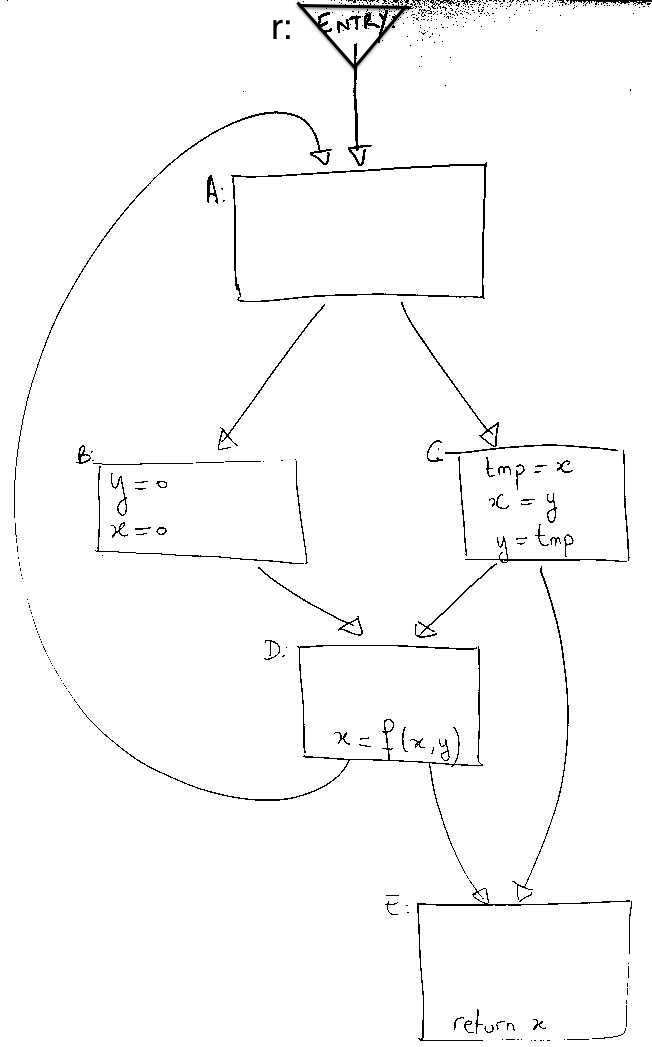
\includegraphics[width=5cm]{initial.jpg}
\caption{\label{fig:classical_construction_algorithm:examplecfg}Example control flow graph, before
  SSA construction occurs}
\end{figure}

\section{Construction}
\label{sec:classical_construction}

The original construction algorithm for SSA form 
consists of two distinct phases.
\begin{enumerate}
\item \textbf{\phiop\ insertion} performs \textit{live-range splitting} to ensures that any use of a given variable $v$ is reached~\footnote{A program point $p$ is said to be \emph{reachable} by a definition of $v$, if there exists a path in the CFG from that definition to $p$ that does not contain any other definition of $v$.}  by exactly one definition of $v$. 
The resulting live-ranges exhibit the property of having a single definition, which occurs at the beginning of each live-range.
\item \textbf{variable renaming} assigns a unique variable name to each live-range. This second phase rewrites variable names in program statements such that the program text contains only one definition of each variable, and every use refers to its corresponding unique reaching definition.
\end{enumerate}

As already outlined in Chapter \ref{chap:properties_and_flavours},
there are different flavors of SSA with distinct properties.
In this chapter, we focus on the \textit{minimal} SSA form.

\subsubsection*{Join Sets}

Construction of minimal SSA 
requires for each variable $v$ the insertion of \phiops\ at $\join(D_v)$.
Here $D_v$ is the set of nodes that contain definitions of $v$, and,
for a given set of nodes $S$, $\join(S)$ is the set of
\textit{join nodes} of $S$
i.e., nodes in the CFG that can be reached by
two (or more) distinct elements of $S$ using disjoint paths.
Join sets were introduced in Section~\ref{sec:properties_and_flavors:minimal}.

Let us consider some join set examples from the
program in Figure \ref{fig:classical_construction_algorithm:examplecfg}.
\begin{enumerate}
\item $\join(\{B,C\}) = \{D\}$, since it is possible to get from $B$ to $D$
and from $C$ to $D$ along different, non-overlapping, paths.
\item Again, $\join(\{r, A, B, C, D, E \}) = \{A,D,E\}$, since the nodes
$A$, $D$, and $E$ are the only nodes with multiple predecessors in
the program.
\end{enumerate}

 
The original construction for SSA form uses an over-approximation of
join sets, the
\emph{iterated dominance frontier}, $\iDF(S)=\join(S\cup
\{r\})$, i.e.\ it assumes an \emph{implicit} definition of every
variable at the entry node $r$.
The iterated dominance frontier is the limit $DF_{i\rightarrow\infty}(S)$
of the sequence:
$$\begin{array}{lll}
\DF_1(S) & = & \DF(S)\\
\DF_{i+1}(S) & = & \DF\left(S\cup \DF_i(S)\right)
\end{array}$$

% described dominance frontiers? In chapter 2?
Recall the definition of dominance frontiers from Section~\ref{sec:properties_and_flavors:minimal}.
Informally, the dominance frontier of a node $A$, $\DF(A)$,
is the border of the CFG region that is dominated by $A$.
Also note that $\DF$ is defined over individual nodes, 
but for simplicity of presentation, we overload it to 
operate over sets of nodes too, i.e.\ 
$\DF(S) = \bigcup_{s\in S} \DF(s)$.

\subsubsection*{\phiop\ Placement}

This concept of dominance frontiers 
naturally leads to a
straightforward approach that places \phiops\
on a per-variable basis.
For a given variable $v$, we place \phiops\ at the
iterated dominance frontier $\iDF(D_v)$ where
$D_v$ is the set of nodes containing definitions of $v$.
This leads to the construction of a form that has 
the dominance property, i.e. where each variable's definition dominates its entire live-range.

Consider again our running example from Figure 
\ref{fig:classical_construction_algorithm:examplecfg}. The set of nodes containing definitions
of variable
$x$ is $\{ B,C,D \}$. The iterated dominance frontier of this set
is $\{ A, D, E \}$. Hence we need to insert 
\phiops\ for $x$ at the beginning of nodes $A$, $D$, and $E$.
Figure \ref{fig:classical_construction_algorithm:examplecfg_varx} shows the example CFG program
with inserted \phiops\ for $x$ marked in red.



As far as the actual algorithm for \phiops\ insertion
is concerned, we will assume that the dominance
frontier of each CFG node is precomputed and that the iterated dominance frontier is computed just-in-time, as the algorithm proceeds.
The algorithm works by inserting \phiops\ iteratively
using a worklist of definition points, and flags (to avoid multiple
insertions). The corresponding pseudo-code for
\phiop\ insertion is given in
Algorithm~\ref{alg:classical_construction:phi_insertion}.


The worklist of nodes $W$ is used to record definition points that the
algorithm
has not yet processed, i.e.\ it has not yet inserted \phiops\ at their dominance
frontiers.
Because a \phiop\ is itself a 
definition, it may require further \phiops\ to be inserted.
This is the cause of node insertions into the worklist $W$ during
iterations of the inner loop in Algorithm 
\ref{alg:classical_construction:phi_insertion}.
Effectively, this is the just-in-time construction of
the iterated dominance frontier.


The flags array $I$ is used to avoid repeated insertion of \phiops\
at a single node. Dominance
frontiers
of distinct nodes may intersect, e.g.\ in the example CFG in Figure
\ref{fig:classical_construction_algorithm:examplecfg},
$\DF(B)$ and $\DF(C)$ both contain $D$. 
Once a \phiop\ for a particular variable has been
inserted at a node,
there is no need to insert another, since a single \phiop\ per
variable handles all incoming definitions of that variable to that node.

Table \ref{tab:classical_construction:walkthru} 
gives a walk-through example of Algorithm 
\ref{alg:classical_construction:phi_insertion}.
It shows the stages of execution for a single iteration of
the outermost for loop, which is inserting \phiops\
for variable $x$.
At the beginning, the CFG looks like Figure \ref{fig:classical_construction_algorithm:examplecfg}.
At the end, when all the \phiops\ for $x$ have
been placed, then the CFG looks like Figure \ref{fig:classical_construction_algorithm:examplecfg_varx}.

\begin{algorithm}
\Begin{
 $W \leftarrow \{ \}$ : set of basic blocks\;
 $I \leftarrow \{ \}$ : set of basic blocks\;
 \For{$v$ : variable names in original program}{
  \For{$d \in D_v$ }{
    \textbf{let} $B$ be the basic block containing $d$\;
     $W \leftarrow W \cup \{ B \}$\;
  }
  \While{$W \neq \{\}$}{
   remove a basic block $X$ from $W$\;
   \For{$Y : \mbox{basic block} \in \mathrm{DF}(X)$}{
    \If{$Y \not\in I$}{
        add $v \leftarrow \phi(...)$ at entry of $Y$\;
        $I \leftarrow I \cup \{ Y \}$\;
        \If{$Y \notin D_v$}{
          $W \leftarrow W \cup \{ Y \}$\;
        }
     }
    }
  }
}
}
\caption{\label{alg:classical_construction:phi_insertion}Standard algorithm for inserting $\phi$-functions}
\end{algorithm}


\begin{table}
\begin{center}
\begin{tabular}{r|c|c|c|c}
\textbf{while loop \#} & $X$ & $\textrm{DF}(X)$ & $I$         & $W$\\ \hline
-                      & -   & -                & $\{\}$      & $\{B,C,D\}$ \\
0                      & $B$ & $\{D\}$          & $\{D\}$     & $\{C,D\}$ \\
1                      & $C$ & $\{D,E\}$        & $\{D,E\}$   & $\{D,E\}$ \\
2                      & $D$ & $\{E,A\}$        & $\{D,E,A\}$ & $\{E,A\}$\\
3                      & $E$ & $\{\}$           & $\{D,E,A\}$ & $\{A\}$\\
4                      & $A$ & $\{A\}$          & $\{D,E,A\}$ & $\{\}$\\ \hline
\end{tabular}
\end{center}
\caption{\label{table:classical_construction:walkthru}Walk-through of
  placement of \phiops\ for variable $x$ in example CFG}
\end{table}

\begin{figure}
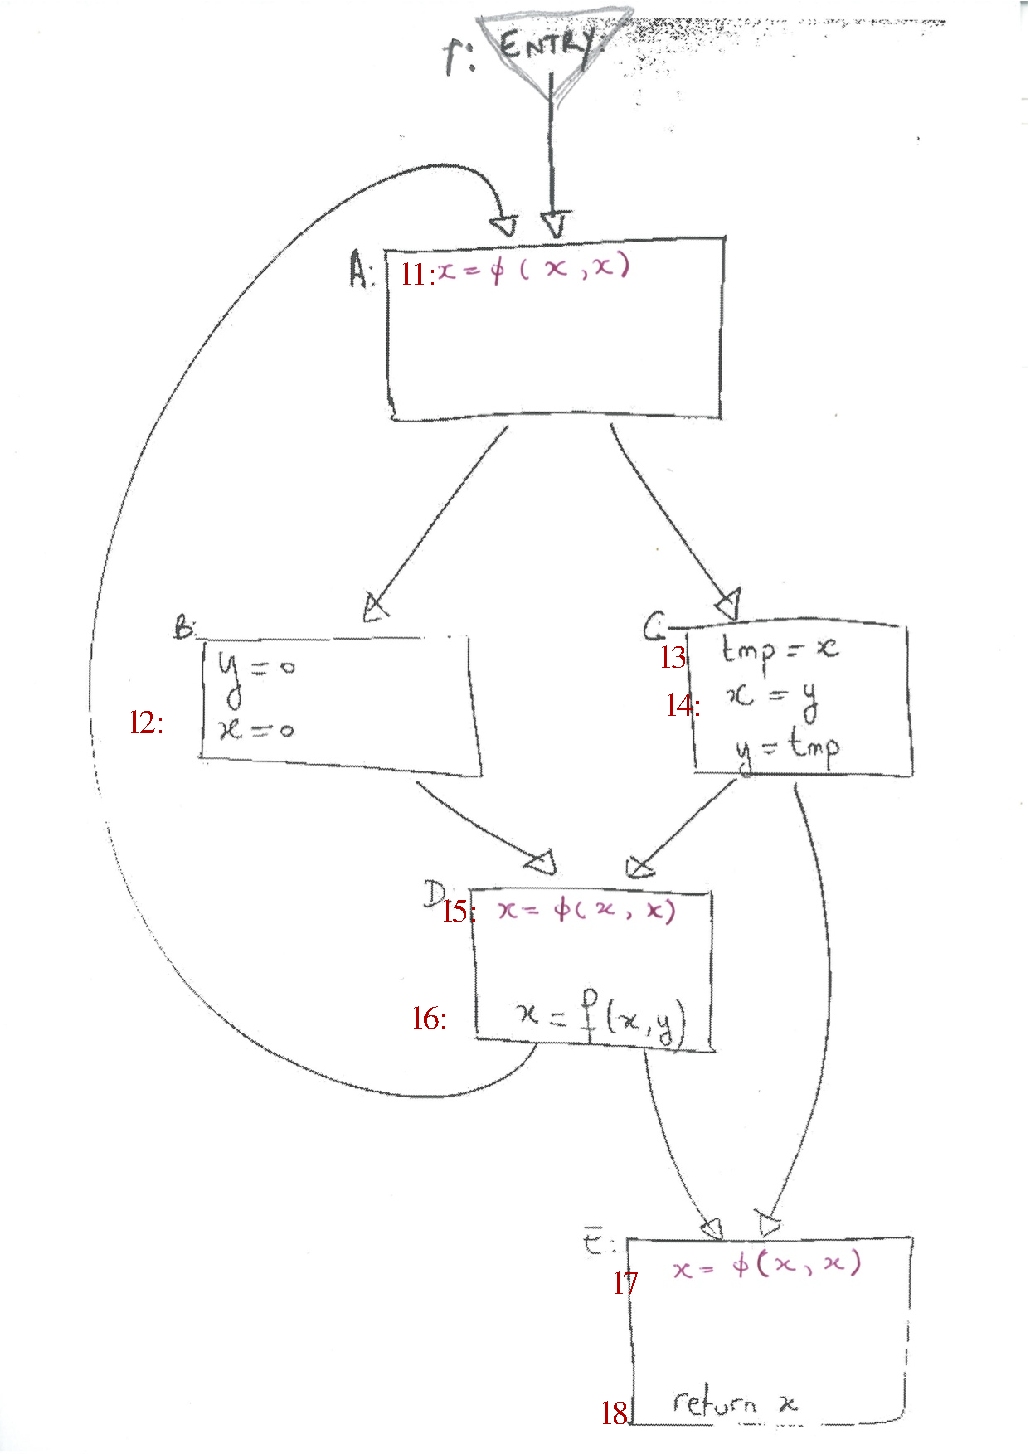
\includegraphics[width=5cm]{ssa_variablex_label.pdf}
\caption{\label{fig:classical_construction_algorithm:examplecfg_varx}Example control flow graph, including
inserted \phiops\ for variable $x$
}
\end{figure}

Providing the dominance tree as a given, the computation of the dominance frontier is quite straight-forward. As illustrated by Figure~\ref{fig:classical_construction_algorithm:iDF}, this can be understood using the DJ-graph notation. The skeleton of the DJ-graph is the dominator tree of the CFG that makes the $D$-edges. This is augmented with $J$-edges (join edges) that correspond to all edges of the CFG which source do not dominate its destination. A $DF$-edge (dominance frontier edge) is an edge which destination is in the dominance frontier of its source. By definition, there is a $DF$-edge $(a,b)$ between every CFG nodes $a$, $b$ such that there is a CFG-path from $a$ to $b$ but $a$ does not dominate $b$. 
In other-words, for each  $J$-edge $(a,b)$, all ancestors (including $a$) that do not dominate $b$ have $b$ in their dominance frontier. This leads to the pseudo-code given in Algorithm~\ref{alg:classical_construction:df}. The iterated dominance frontier is nothing else than the transitive closure of the dominance frontier and we can define the $iDF-graph$ as the transitive closure of the $DF$-graph. 

We can compute the iterated dominance frontier for each variable independently, as proposed in this chapter, or ``cache'' it to avoid multiple computation of the iterated dominance frontier of the same node. This leads to more sophisticated algorithms detailed in Chapter~\ref{chap:alternative_ssa_construction_algorithms}.

\begin{figure}
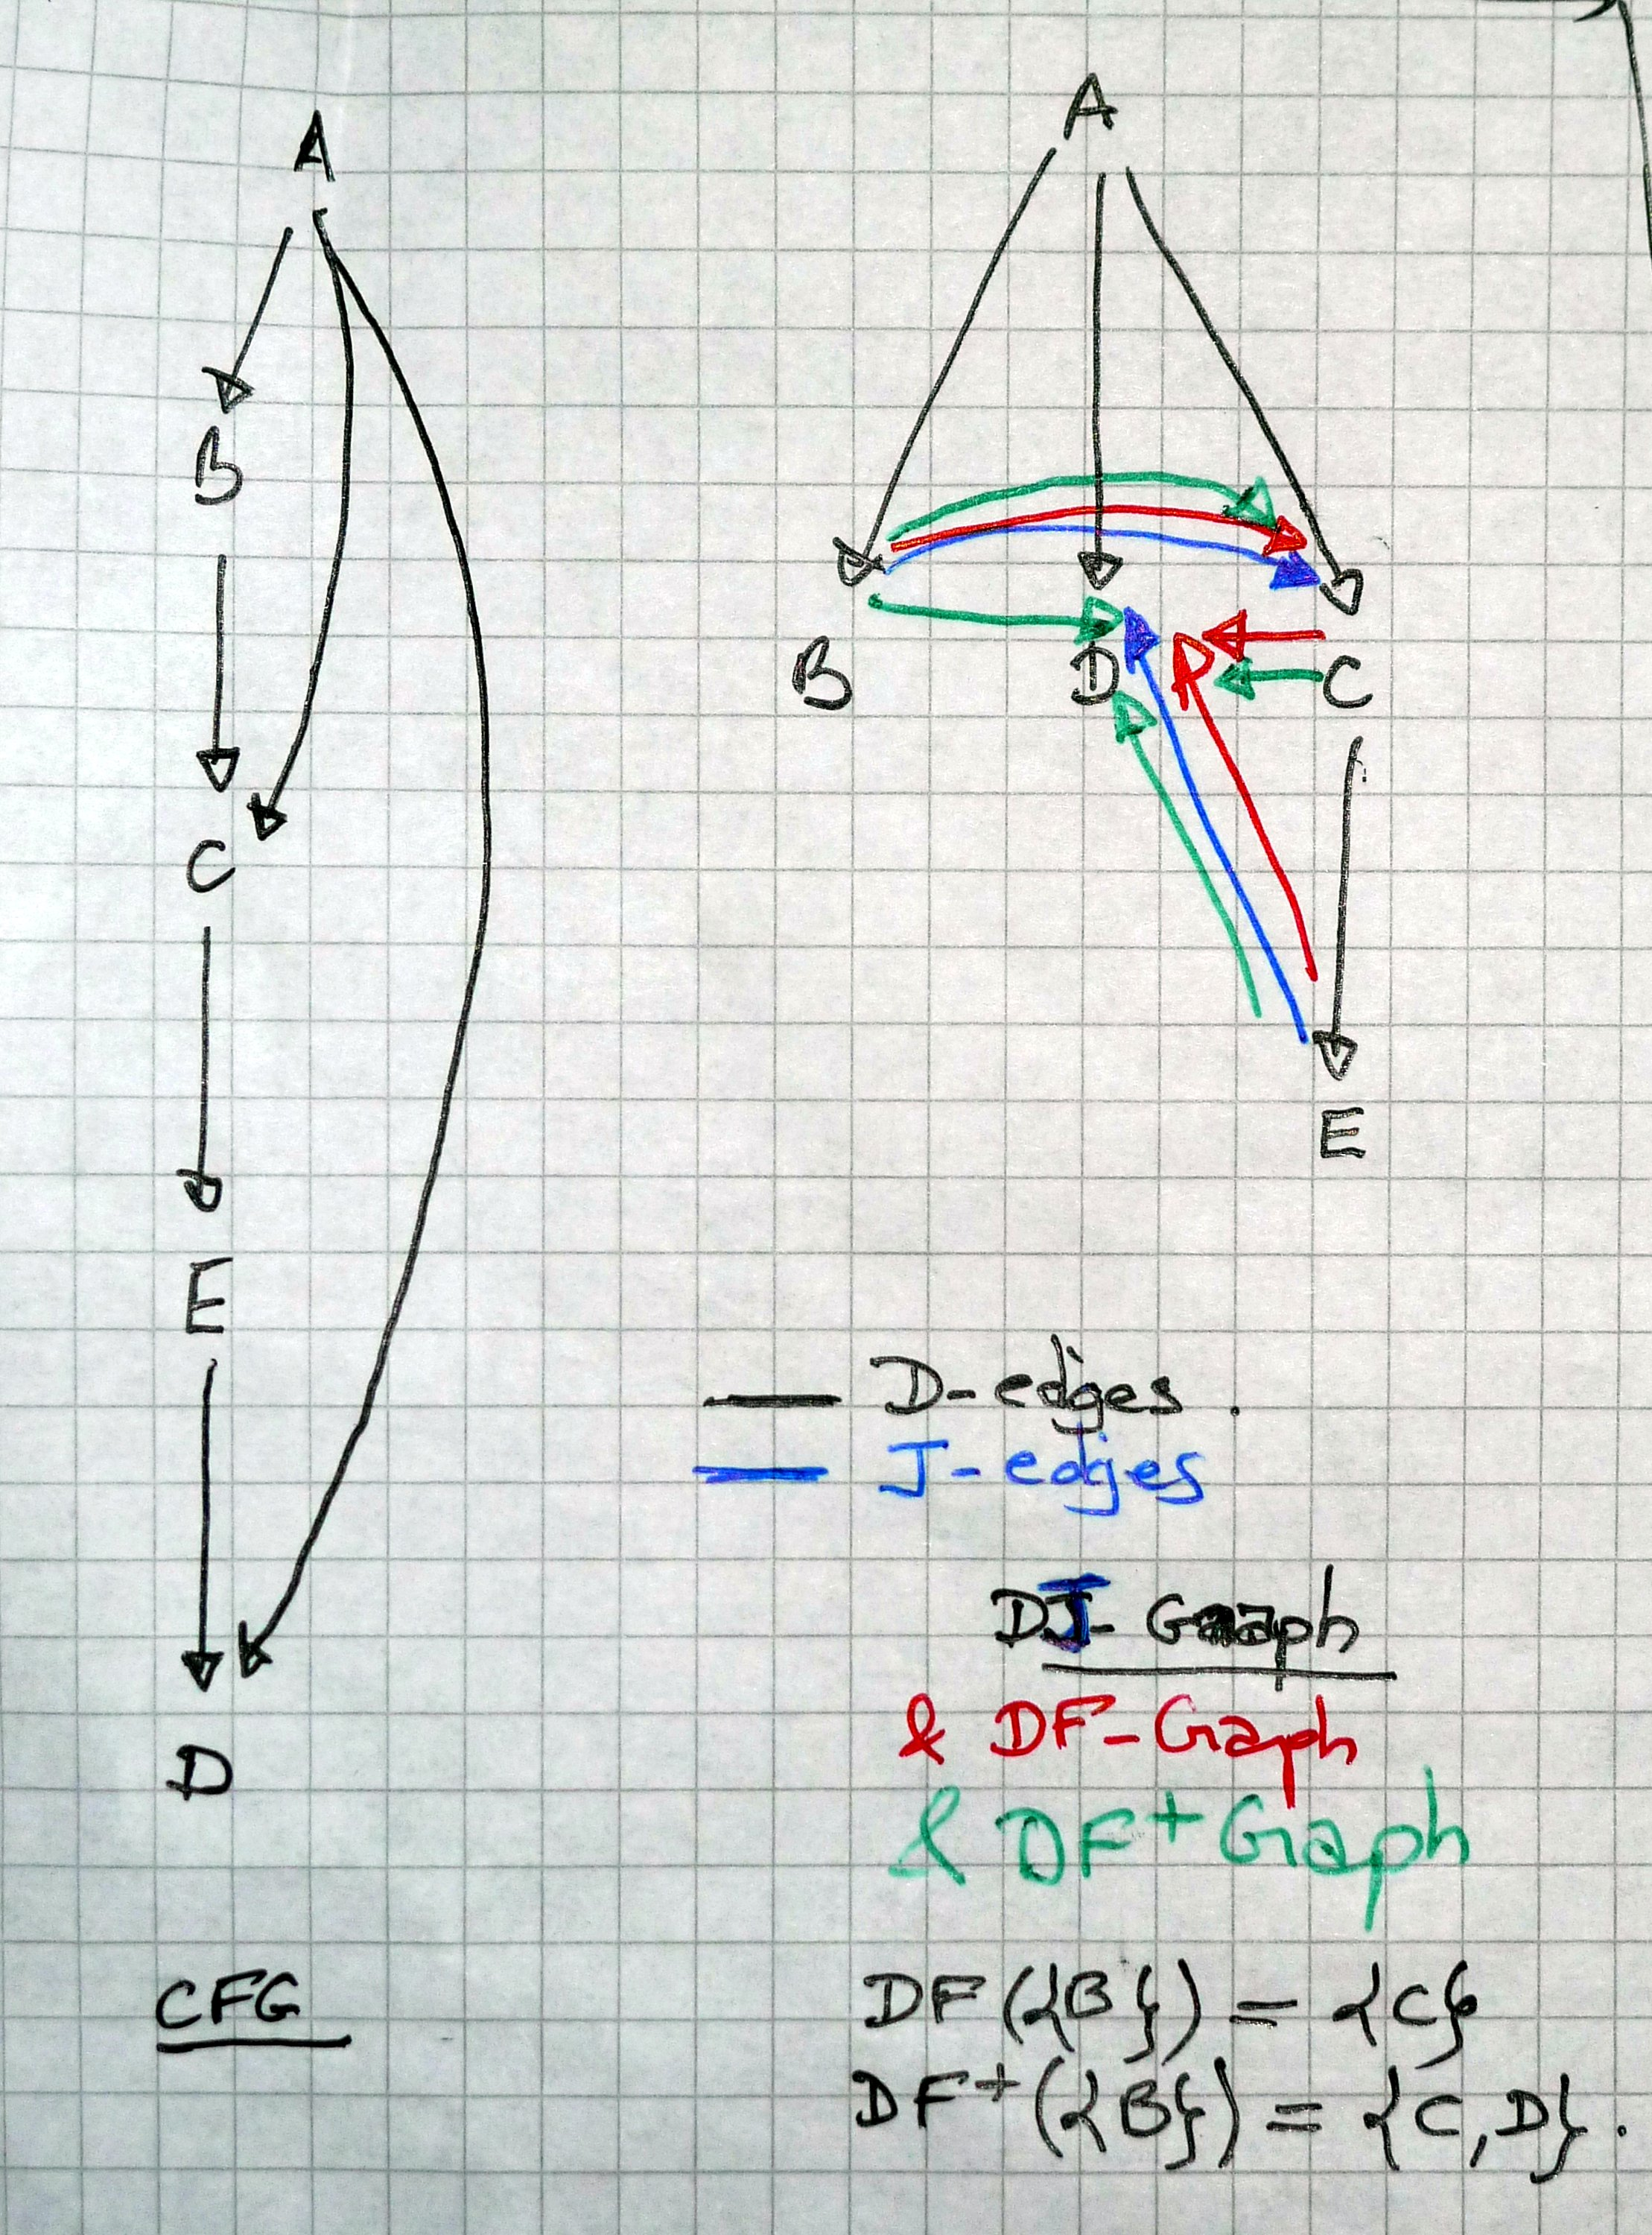
\includegraphics[width=0.5\textwidth]{iDF.jpeg}
\caption{An example CFG and it corresponding DJ-graph, DF-graph and iDF-graph}
\end{figure}

\begin{algorithm}
\Begin{
 \For{$(a,b) \in cfgEdges$}{
  \While{not a dominate b}{
     $\DF(a) \leftarrow \DF(a) \cup b$\;
     $a \leftarrow \mathrm{iDom}(a)$\;
  }
 }
}
\caption{\label{alg:classical_construction:df}Algorithm for computing the dominance frontier of each CFG node}
\end{algorithm}



Once \phiops\ have been inserted using this algorithm, the program may
still contain several definitions per variable, however now there is a
single definition statement 
in the CFG that reaches each use. 
It is conventional to treat the each variable use in a \phiop\
as if it actually occurs on the corresponding incoming edge or at the end of the
corresponding predecessor node.
If we follow this convention,  
% Moreover, with the following semantics for \phiops\ where its
% variable uses are considered to be on the corresponding predecessor
% basic blocks,
then use-def chains are aligned with the CFG dominance tree.
In other words,
\emph{the single definition that reaches each use dominates that use}.

\subsubsection*{Renaming Phase}
\newcommand\reachingDef[1]{#1.\mathrm{reachingDef}}
To obtain the desired property of a static single assignment per variable,
it is necessary to perform \textbf{variable renaming}, which
is the second phase in the SSA construction process.
\phiop\ insertions have the effect of splitting the live-range(s) of each original variable into pieces. The variable renaming phase associates to each individual live-range a new variable name, also called \emph{version}.
Algorithm \ref{alg:classical:renaming} presents the pseudo-code
for this process.
Because of the dominance property outlined above,
it is straightforward to rename variables
using a depth-first traversal of the dominance tree.
During the traversal, for each variable $v$, it is necessary to
remember its unique reaching version's definition at some point $p$ in the graph. This corresponds to the closest definition dominating $p$.
In Algorithm \ref{alg:classical:renaming}, we compute and cache the 
reaching definition for $v$ in the variable field $\reachingDef{v}$ that is updated as the algorithm traverses the dominator tree of the SSA graph.

The variable renaming algorithm translates our running example 
from Figure~\ref{fig:classical_construction_algorithm:examplecfg}.
into the SSA form of Figure
\ref{fig:classical_construction_algorithm:renaming}.
Table \ref{table:classical_construction_algorithm:renaming} 
gives a walk-through example of this algorithm.

\begin{table}
\begin{tabular}{c|c|l}
Basic-block & operand &  reachingDef\\ \hline
Entry & use of $l_1$ & $\bot$\\
$A$ & def of $l_1$ &  $\bot$ then $x_1$\\
$B$ & def of $l_2$ &  $x_1$ then $x_2$\\
$B$ & use of $l_5$ & $x_2$\\
$C$ & use of $l_3$ & $x_2$ updated into $x_1$\\
$C$ & def of $l_4$ &  $x_1$ then $x_3$\\
$C$ & use of $l_5$ & $x_3$\\
$D$ & def of $l_5$ & $x_3$ updated into $x_1$ then $x_4$\\
$D$ & use of $l_6$ & $x_4$\\
$D$ & def of $l_6$ & $x_4$ then $x_5$\\
$D$ & use of $l_1$ & $x_5$\\
$D$ & use of $l_7$ & $x_5$\\
$E$ & def of $l_5$ & $x_5$ then $x_6$\\
$E$ & use of $l_8$ & $x_6$
\end{tabular}
\caption{\label{table:classical_construction_algorithm:renaming}Walkthrough of renaming for variable $x$ in example CFG}
\end{table}

\begin{figure}
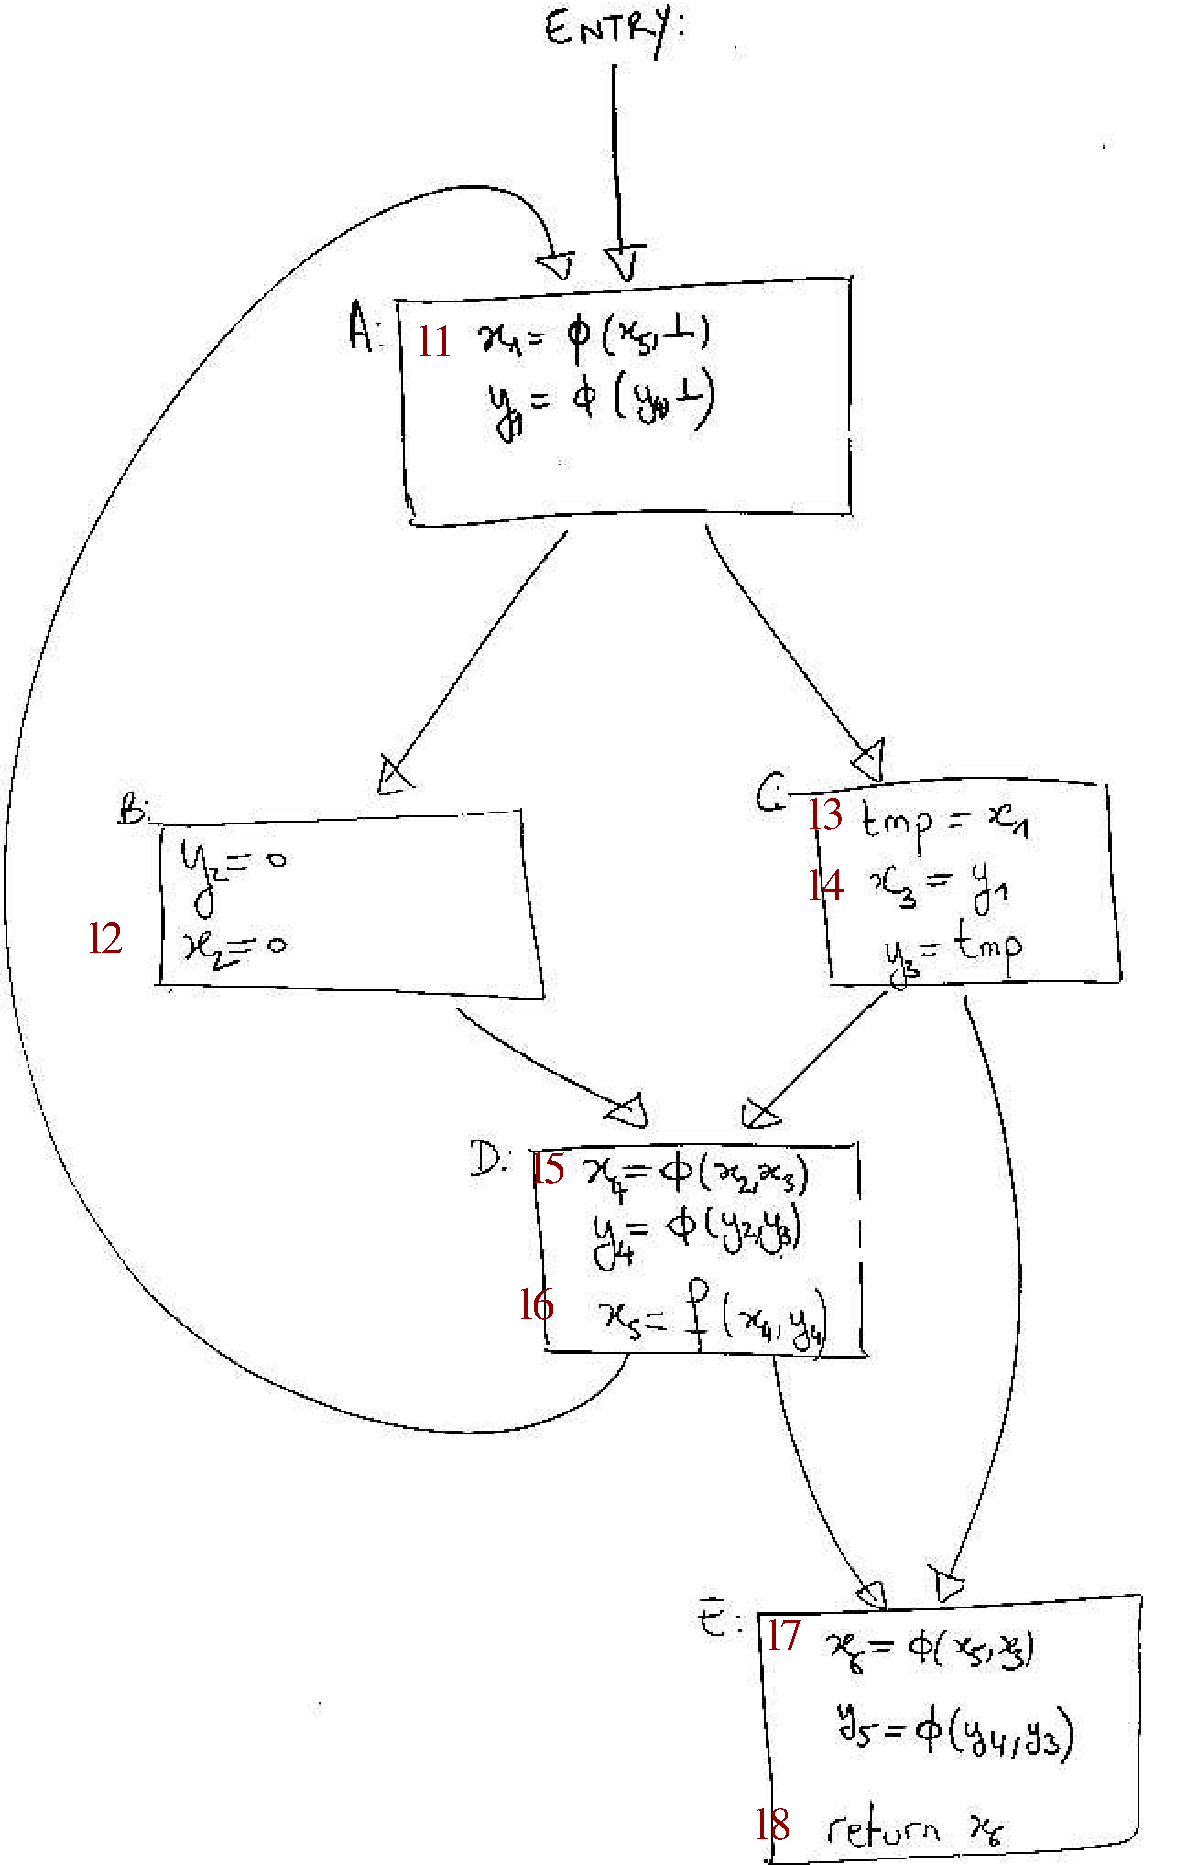
\includegraphics[width=0.5\textwidth]{renaming_label.pdf}
\caption{\label{fig:classical_construction_algorithm:renaming} SSA form of the example of Figure~\ref{fig:classical_construction_algorithm:examplecfg}}
\end{figure}

\begin{algorithm}
%proc renaming:
\Begin{
\tcc{rename variable definitions and uses to have one definition per
  variable name}
\ForEach{v : Variable}{
    $\reachingDef{v} \leftarrow \bot$\;
}
\ForEach{ B : basic Block in depth-first search preorder traversal of the dominance tree}{
  \ForEach{ i : instruction in linear code sequence of B}{
      \ForEach{v : variable used as a source operand on right-hand
        side of  non-\phiop\ i}{
        $\mathrm{updateReachingDef}(v,i)$\;
        replace this use of $v$ by $\reachingDef{v}$ in $i$\;
      }
      \ForEach{ v : variable defined by i, which may be a \phiop}{
        $\mathrm{updateReachingDef}(v,i)$\;
        create fresh variable $v'$\;
        replace this definition of $v$ by $v'$ in $i$\;
        $\reachingDef{v'} \leftarrow \reachingDef{v}$ \;
        $\reachingDef{v} \leftarrow v'$\;
      }
  }
  \ForEach{f: \phiop\ in a successor of B}{
      \ForEach{ v : variable used as a source operand on right-hand
        side of f}{
        $\mathrm{updateReachingDef}(v,f)$\;
        replace this use of $v$ by $\reachingDef{v}$ in $f$\;
      }
 }
}
}
\caption{\label{alg:classical:renaming}Renaming algorithm for second
  phase of SSA construction}
\end{algorithm}

\begin{procedure}
\KwData{$v$ : variable from program}
\KwData{$i$ : instruction from program}
\Begin{
  \tcc{search through chain of definitions for v until we find the
    closest definition that dominates i, then update $\reachingDef{v}$
    in-place with this definition}
  $r \leftarrow \reachingDef{v}$\;
  \While{ not ($r==\bot$ or definition($r$) dominates $i$)}{
    $r \leftarrow \reachingDef{r}$\;
  }
  $\reachingDef{v} \leftarrow r$\;
}
\caption{updateReachingDef(v,i) Utility
  function for SSA renaming\label{alg:classical:updateRD}}
\end{procedure}

% Some paragraphs summarizing similarities / diffs between this
% algorithm and standard stack-based renaming algorithm.
This renaming algorithm uses a single $\mathrm{reachingDef}$ slot 
per variable to store the in-scope, `new' variable name (version) for each
variable used in the un-renamed program. An equivalent approach uses a stack that stores all versions that dominate the current program point. 
A stack value is pushed when a variable definition is
processed (while we explicitly update the reachingDefs field at this point).
The top stack value is peeked when a variable use is encountered
(we read from the reachingDefs field at this point).
Multiple stack values may be popped when moving to a different node
in the dominator tree 
(we always check whether we need to update the reachingDefs field
before we read from it).

While the slot-based algorithm requires more memory, it can take advantage of an existing variable's working field, and be more efficient in practice. 

\subsubsection*{Summary}

Now let us review the flavour of SSA form that this simple
construction algorithm produces. We refer back to several
SSA properties that were introduced in
Chapter \ref{chap:properties_and_flavours}.

\begin{itemize}
\item It is \textit{minimal}, see Section \ref{sec-prop-minimal}.
After the \phiop\ insertion phase,
but before variable renaming, the CFG contains the minimal 
number of inserted \phiops\ to achieve the property that exactly
one definition of each variable $v$ reaches every point in the graph.
\item It is \textit{not pruned}, see Section \ref{sec-prop-pruned}.
Some of the inserted \phiops\
may be dead, i.e.\ there is no explicit use of the variable subsequent
to the \phiop.
\item It is \textit{conventional}, see Section \ref{sec-prop-conventional}.
The transformation that renames all $\phi$-related variables into a
unique representative name, and then removes all \phiops\ is a correct SSA-destruction algorithm.
\item Finally, it has the \textit{dominance} property, see Section
\ref{sec-prop-dominance}.
Each variable use is dominated by its unique definition. This is due to the use during the $\phi$-placement phase of iterated dominance frontier instead of join set. Whenever the iterated dominance frontier of the set of definition points of a variable differs from the join set, then at least one program point can be reached both by $r$ (the entry of the CFG) and one of the definition points. In other words, as in Figure~\ref{fig:classical_construction_algorithm:examplecfg}, one of the uses of the \phiop\ inserted in block $A$ for $x$ does not have any actual reaching definition that dominates it. This corresponds to the undef value used to initialize reachingDef in the renaming phase pseudo code. Actual implementation can use NULL value, create a fake undefined variable at the entry of the CFG, or create on the fly undef pseudo operations just before the concerned used. We choose to use in this book the undef value, represented with the $\undef$ sign.
\end{itemize}


\section{Destruction}
\label{sec:classical_construction_algorithm:destruction}

SSA form is a 
sparse representation of program information,
which enables simple, efficient code analysis and optimization.
Once we have completed SSA based optimization passes,
and certainly before code generation,
it is necessary to eliminate \phiops\ since these
are not executable machine instructions.
This elimination phase is known as \textit{SSA destruction}. 

As a freshly constructed SSA code is conventional, its destruction is straightforward.
%\emph{Khedker calls this CSSA for canonical SSA - from earlier ref?}
%FAB: never heard about this and google does not help. C-SSA is for conventional SSA according to Sreedhar. Khedker refers to the paper of Sreedhar for SSA destruction. So I guess he made a mistake.
One simply has to rename all 
$\phi$-related variables (source and destination operands of
a single \phiop\ are related)
into a unique representative variable.
Then each \phiop\ should have identical names for all its operands,
and thus can be removed to coalesce the related live-ranges.

We refer to a set of $\phi$-related variables as
an \textit{SSA-web}. Conventional SSA is defined as a flavor under which each SSA-web is interference free. The discovery of SSA-webs can be performed efficiently 
using the classical \textit{union-find} algorithm 
with a disjoint-set data structure,
which keeps track of a set of elements
partitioned into a number of disjoint (non-overlapping) subsets.
The SSA-webs discovery algorithm is presented in 
Algorithm \ref{alg:ssadestruction:find-webs}.

\begin{algorithm}
%% proc find_webs
%% // find the ssa web of each variable
\Begin{
\For{each variable $v$}{
  $\mathrm{ssaweb}(v) \leftarrow \{v\}$;
}
\For{each instruction of the form $a_{\mathrm{dest}} = \phi(a_1,\ldots,a_n)$}{
  \For{each source operand $a_i$ in instruction}{
     union$(\mathrm{ssaweb}(a_{\mathrm{dest}}),\mathrm{ssaweb}(a_i))$
  }
}
}
\caption{\label{alg:ssadestruction:find-webs}The SSA-webs discovery algorithm, based on the union-find pattern}
\end{algorithm}


While freshly constructed SSA code is conventional, 
this may not be the case after optimizations 
such as copy propagation have been performed.
Going back to conventional SSA form implies the insertion of copies.
{\emph FIXME: we need to talk about parallel copies at some points. You mention in the vanilla chapter the fact that phi are to be executed in parallel. An option is to explain the parallel semantics in the vanilla chapter using parallel copies on incoming edges. Up to you.}

The simplest (although not the most efficient) way to destroy non-conventional SSA form is to split all \textit{critical edges}, and then replace \phiops\ by parallel copies at the end of predecessor basic blocks.
A critical edge is an edge from a node with several successors to a node with several predecessors.
The process of splitting an edge, say $(b_1,b_2)$,
involves replacing edge $(b_1, b_2)$ by (i) an
edge from $b_1$ to a freshly created basic block 
and by (ii) another edge from this fresh basic block to $b_2$. 
Algorithm \ref{alg:ssadestruction:splitting} presents
the corresponding pseudo-code.

\begin{algorithm}
\Begin{
 \ForEach{$B$: basic block of the CFG}{
   \Let{$\mathrm{PC}_0$ be $() \leftarrow ()$, an empty parallel copy instruction}\;
   insert $\mathrm{PC}_0$ immediately  after the \phiops\ at the beginning of $B$\;
   \Let{$(B_1,\ldots,B_n)$ be the list of predecessor blocks of $B$}\;
   \ForEach{$B_i$}{
     \Let{$\mathrm{PC}_i$ be $() \leftarrow ()$, an empty parallel copy instruction}\;
     \If{$B_i$ has several successors}{
       create fresh empty basic block $B'_i$;
       replace edge $B_i \rightarrow B$ by edges $B_i \rightarrow B'_i$ and $B'_i \rightarrow B$;
       insert $PC_i$ in $B'_i$;
     }
    \Else{
       append $PC_i$ at the end of $B_i$;
     }
   }
   \ForEach{\phiop\ at the entry of $B$ of the form $a_0=\phi(B_1:a_1,\ldots,B_n:a_n)$}{
     \Let{$a'$ be a freshly created variable}\;
     add copy $a_0 \leftarrow a'$ to $\mathrm{PC}_0$\;
     replace $a_0$ by $a'$ in the \phiop\;
     \ForEach{$a_i$ (argument of the \phiop\ corresponding to $B_i$)}{
       add copy $a' \leftarrow a_i$ to $\mathrm{PC}_i$;
       replace $a_i$ by $a'$ in the \phiop;
     }
     remove \phiop \tcc{otherwise get conventional SSA}
  }
}
}
\caption{\label{alg:ssadestruction:splitting}Critical Edge Splitting Algorithm for destruction of non-conventional SSA form}
\end{algorithm}


Even this extremely conservative SSA destruction algorithm
can potentially lead to potential bugs,
particularly at the code generation stage.
It is essential to ensure that it is possible
to append a copy operation at the very end of a basic block.
This would, for example, be problematic in the situation 
where the jump at the end of the basic block
defines a variable used in the following \phiop,
(such as a Jump-And-Set instruction).
Care must be taken with duplicated edges, i.e.\
when the same basic block appears twice in the list of predecessors.
This can occur after CFG structural optimizations like
dead code elimination or empty block elimination.
In such case, the edges should be considered as critical and then split.

We stress that the above destruction technique has several drawbacks: first because of specific architectural constraints, region boundaries, or exception handling code, the compiler might not permit the splitting of a given edge; second, the resulting code contains many temporary-to-temporary copy operations. In theory, reducing the frequency of these copies is the role of the coalescer during the register allocation phase. A few memory and time-consuming existing coalescing heuristics mentioned in Chapter~\ref{chap:register-allocation} can handle the removal of these copies effectively. Coalescing can also, with less effort, be performed prior to the register allocation phase. As opposed to a (so-called conservative) coalescer during register allocation, this \emph{aggressive} coalescing would not cope with the interference graph colorability. Further, the process of copy insertion itself might take a substantial amount of time and might not be suitable for dynamic compilation. The goal of Chapter~\ref{chap:alternative-destruction} is to cope both with non-splittable edges and difficulties related with SSA destruction at machine code level, but also aggressive coalescing in the context of resource constrained compilation.

Once \phiops\ have been replaced by parallel copies, we need to sequentialize the parallel copies, i.e.\ replace them by a sequence of simple copies. This phase can be performed immediately after SSA destruction or later on, perhaps even after register allocation (see Chapter~\ref{chap:register_allocation}). It might be useful to postpone the copy sequentialization since it introduces arbitrary interference between variables. As an example, $(a_1,b_1)\gets (a_2,b_2)$ can be sequentialized into $a_1\gets a_2;\ b_1\gets b_2$ which would make $b_2$ interfere with $a_1$ while the other way round $b_1\gets b_2;\ a_1\gets a_2$ would make $a_2$ interfere with $b_1$ instead.

If we still decide to replace parallel copies into a sequence of simple copies immediately after SSA destruction described in this chapter (with no copy propagation / coalescing in between), this is straightforward: as no variable appears as both a source and a destination (either all the sources or all the destinations are freshly created variables), any order is correct. Chapter~\ref{chapter:alternative_ssa_destruction_algorithm} will provide the pseudo-code that is required after coalescing have been performed and Chapter~\ref{chapter:register_allocation} will deal with the case involving register-allocated code.

\section{Turning general SSA into minimal/conventional/pruned/dominance property}

As discussed in Chapter~\ref{chapter:properties_and_flavours},
SSA comes in different flavors. 
% It may or may not be conventional
% (each SSA web is interference free); 
% it may or may not fulfill the 
% dominance property (each variable 
% definition dominates all its uses); 
% it may or may not be pruned (does 
% not contain any dead \phiop); it 
% may or may not be minimal (there 
% is no ``identity'' \phiops).
This section describes  algorithms that transform SSA
code
into the desired flavor.

Making SSA \textit{conventional} corresponds exactly to the first phase of SSA destruction (described in Section~\ref{sec:classical_destruction}) that splits critical edges and introduces parallel copies (sequentialized later on or on the fly) around \phiops. As already discussed, this straightforward algorithm has several drawbacks addressed in Chapter~\ref{chapter:chapter:alternative_ssa_destruction_algorithm}.

Making SSA strict, i.e.\ fulfill the dominance property, is as `hard' as constructing SSA. Of course, a pre-pass can detect the variables that have definitions that do not dominate their uses. Then there are several possible single-variable \phiops\ insertion algorithms (see Chapter~\ref{chapter:alternative_ssa_construction_algorithms}) that can be used to patch up the SSA, by restricting attention to the set of non-conforming variables. The renaming phase can also be used with the same filtering process. As the number of variables to repair might be a small proportion of all variables, a costly traversal of the whole program can be avoided by building the def-use chains (the non dominating ones) during the detection phase. Renaming can then be done on a per-variable basis or better (if pruned SSA is preferred) the reconstruction algorithm presented in Chapter~\ref{chapter:repair_maintain_ssa_after_optimization} can be used both for \phiops\ placement and renaming.

The construction algorithm described above in
Section \ref{sec:classical_construction} does not
build pruned SSA form. It can easily be modified to 
build \textit{semi-pruned SSA} form by simply filtering out the local variables, i.e.\ variables which have definitions that dominate their uses and appear only in the same basic block. Then, if liveness information is available prior to the construction, it can be used to filter out the insertion of \phiops\ wherever the variable is not live.
If the original liveness information is not available, pruning SSA form is equivalent to a dead-code elimination pass. As use-def chains are explicitly provided by SSA form, it simply relies on marking actual uses (non-\phiops\ ones) as useful and propagating backward through \phiops\ usefulness. This leads to the following pseudo-code:

\begin{algorithm}
\begin{verbatim}
stack = ()
foreach I: instruction of the CFG in dominance order
  if I of the form "a=phi(...)"
    mark a has useless
  else I of the form "...=f(a1,...,an)"
    foreach ai defined by a phi function
      mark ai as useful
      stack.push(ai)
while a := stack.pop
  let I: "a=phi(a1,...,an)" be the phi-function that defines a
  foreach ai marked as useless
    mark ai as useful
    stack.push(ai)
foreach I: phi instruction of the form a=phi(...)
  if a marked as useless then delete I  
\end{verbatim}
\label{alg:classical_construction_algorithm:pruning}
\end{algorithm}
Construction of Minimal SSA comes with the price of a sophisticated algorithm involving iterated dominance frontier. 
Still, \phiops\ placement could be done pessimistically, as described further, on each CFG nodes along the live-ranges of the variables (or at every basic-block if we are extremely lazy or simply do not want SSA to be pruned). 
Also, code transformations such as code motion, CFG modifications, can make a minimal SSA non minimal.
Actually, minimality can be obtained/recovered using copy propagation whenever the CFG is reducible. 
To be efficient (as otherwise as many iterations as the maximum loop depth might be necessary), def-use chains should be computed. 
As already mentioned in Chapter~\ref{chapter:properties_and_flavours}, copy propagation can break the dominance property by propagating variable $a$ through \phiops\ of the form $a'=\phi(a_1,...,a_n)$ where $a_i$ are either equal to $a$ or $\undef$. 
If we want to avoid breaking the dominance property we simply have to avoid the use of this simplification rule that involves $\undef$. 
A more interesting rule is the one that propagates $a$ through a \phiop\ of the form $a'=\phi(a_1,...,a_n)$ where $a_i$ is either equal to $a$ or $a'$. 
``Identity'' \phiops\ can be simplified this way from inner to outer loops. 
Actually, when the CFG is reducible, this leads to minimal SSA. 
The underlying reason for that is that the def-use chain of a given variable is in this context a sub graph of a reducible graph: 
all nodes but those that can be reached by two different paths (from actual non \phiops\ definitions) can be simplified using iteratively $T1$ (merge of a node to its unique predecessor) or $T2$ (removal of self edge) reductions.
More precisely:
\begin{itemize}
\item simplifying any \phiop\ $a'=\phi(a_1,...,a_n)$ such that all $a_i$ are equals corresponds to $T1$ reduction
\item simplifying any \phiop\ $a'=\phi(a_1,...,a_n)$ such that each $a_i$ is either equal to $a'$ or to $a_1$, corresponds to $T2$ followed by $T1$ reduction.
\end{itemize}
This leads to a worklist algorithm in which the worklist stores the nodes that might be simplified. The worklist can be initialized with successors of non-\phiops\ definitions of variables (sources of the graph) -- if we want to stick on the framework of graph reduction --, or simply with all \phiops. Of course, if loop nesting forest is available, worklist can be avoided by traversing the CFG in a single pass from inner to outer loops, and in a topological order within each loop (header excluded)... 
As we believe the main motivation for this approach to be its simplicity, the pseudo-code provided here uses a worklist:

\begin{verbatim}
worklist := ()
foreach I: phi instruction of the program
  worklist.push(I)
  mark I
while worklist is non empty
  unmark I
  I := worklist.shift
  let I be of the form a'=phi(a1,...,an)
  if foreach ai, ai in {a1,a'}
    foreach I': instruction different than I that uses a'
      replaces a' by a1 in I'
      if I' not marked
        mark I'
        worklist.push(I')
\end{verbatim}


\section{Additional reading}

The early literature on SSA form
\cite{cytron89efficient,cytron91efficiently}
introduces both phases of the construction algorithm
we have outlined in this chapter,
and discusses algorithmic complexity on common and worst-case inputs.
These initial discussions trace its ancestry of SSA form back to the
early work on data flow representations by Shapiro and Saint
\cite{shapiro69representation}.

There are numerous published descriptions of alternative algorithms
for SSA construction, in particular for the \phiop\ insertion phase.
The pessimistic approach that first inserts \phiops\ at all control flow merge points and then remove unnecessary ones using simple rewrite rules was proposed by Aycock
and Horspool \cite{aycock00simple}. 

Sreedhar and Gao \cite{sreedhar95linear} pioneered
linear-time complexity construction algorithms based on DJ-graphs.
Their work has since been refined by other researchers.
Chapter \ref{chap:alternative_ssa_construction_algorithms}
explores these more efficient algorithms in depth.

Blech et al \cite{blech05optimizing}
formalize the semantics of SSA, in order to verify
the correctness of SSA destruction algorithms.
Boissinot et al \cite{boissinot09revisiting} review the history of SSA destruction approaches,
and highlight misunderstandings that led to incorrect destruction
algorithms.
Chapter \ref{chap:alternative_ssa_destruction_algorithm} presents
more details on alternative approaches to SSA destruction.

%%% FAB: we should probably move the technical discussions to this part?
Still missing:
\begin{itemize}
\item Semantic chapter (for minimality they have a similar copy-prop algo in the context of functional programming; for construction and dominance notion they have a nice equivalence with functional programming again) 
\item Wolf (J+=J) for join set
\item Maybe a brief history with previous ``incorrect papers''.
\end{itemize}
